
%%%%%%%%%%%%%%%%%%%%%%%%%%%%%%%%%%%%%%%%%%%%%%%%%%%%%%%%%%%%%%%%%%%%%%%%%%%%%%%%%%%%%%%%%%%%%%%%%%%%%%%%%%%%%
\section{Casas-Ibarra parametrization}
\label{sec:casas-ibarra}

In process...
 
{\color{red}
For two scalar singlets, $\boldsymbol{\mathcal{R}}$ can be specified in terms of a single parameter 
\begin{align}
  \boldsymbol{\mathcal{R}}=&
  \begin{pmatrix}
    1 & \cos\theta & \sin\theta\\
    0 & -\sin\theta & \cos\theta\\
    0 &   0        & 1         \\ 
  \end{pmatrix}
\end{align}
and we get
\begin{align}
  h_{i1}=&\frac{\sqrt{m^\nu_2}\cos\theta U^{*}_{i2}+ \sqrt{m^\nu_3}\sin\theta U^{*}_{i3}}%
{\sqrt{\Lambda_1}},\nonumber\\
h_{i2}=&\frac{-\sqrt{m^\nu_2}\sin\theta U^{*}_{i2}+ \sqrt{m^\nu_3}\cos\theta U^{*}_{i3}}%
{\sqrt{\Lambda_2}},
\end{align}
}

in process...

\subsection{Python code for the T13A model}
The numerical implementation of the Casas-Ibarra was:




%%%%%%%%%%%%%%%%%%%%%%%%%%%%%%%%%%%%%%%%%%%%%%%%%%%%%%%%%%%%%%%%%%%%%%%%%%%%%%%%%%%%%%%%%%%%%%
\section{The polarization vectors}
\label{sec:polarization-vectors}
%
The Fourier decomposition of the photon's field with $\omega_k=|\vec{k}|$ is, 
\begin{align}
A^{\mu}(x)=\int\dfrac{d^3k}{\sqrt{2\pi^32\omega_k}}\sum_{r=0}^3\left[\epsilon_r^{\mu}(k)a_r(k)e^{-ik\cdot x} + \epsilon_r^{*\mu}(k)a^{\dagger}_r(k)e^{ik\cdot x}\right]\,,
\end{align}
%
where $\epsilon_0^{\mu}$ is the scalar polarization, $\epsilon_3^{\mu}$ is the longitudinal polarization and $\epsilon_{2,3}^{\mu}$ are the transverse polarization vectors of the photon. Now, if we choose the propagation in the $\vec{k}$ direction, the representation of the polarization vectors $\epsilon_r^{\mu}$ in the particular case of circularly polarization is given by
\begin{align}
\epsilon_0^{\mu} =& (1,0,0,0)\nonumber \\
\epsilon_1^{\mu} =& \dfrac{(0,1,\pm\, i,0)}{\sqrt{2}}= \dfrac{(0,1,r_3\, i,0)}{\sqrt{2}} \nonumber \\
\epsilon_2^{\mu} =& \dfrac{(0,1,\mp\, i,0)}{\sqrt{2}}= \dfrac{(0,1,r_4\, i,0)}{\sqrt{2}} \nonumber \\
\epsilon_3^{\mu} =& (0,0,0,1)\,,
\end{align} 
where in general the parameters $r_3 , r_4$ gives us the two possible choice for the direction of the rotation of the transverse polarization vectors.





%%%%%%%%%%%%%%%%%%%%%%%%%%%%%%%%%%%%%%%%%%%%%%%%%%%%%%%%%%%%%%%%%%%%%%%%%%%%%%%%%%%%%%%%%%%%%%%%%%%%%%%%%%%%%%%%%
\section{ Velocity averaged annihilation cross section $\langle \sigma v \rangle$ }
\label{sec:sigmav}
%
\begin{figure}[h]
\begin{center}
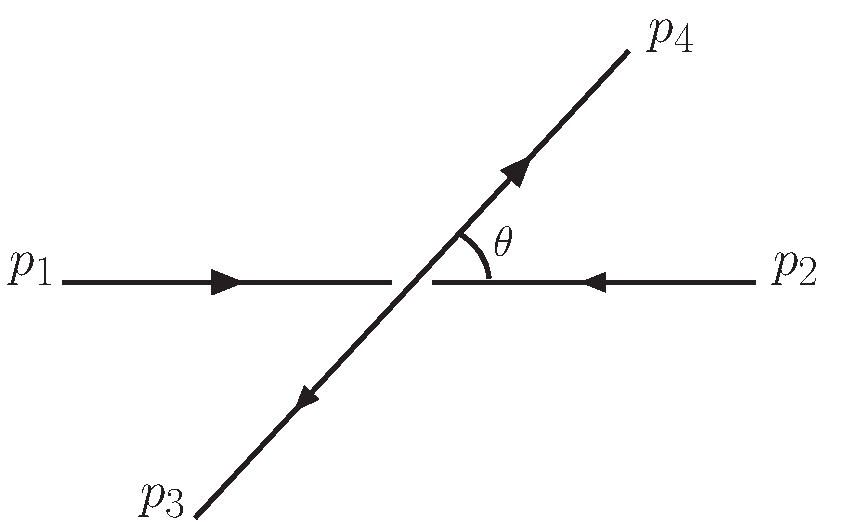
\includegraphics[scale=0.4]{CM}
\end{center}
\caption{Two particles scattering in the center of mass frame.}
\label{fig:cm-frame}
\end{figure}
%
It is known that for an scattering shown in the Fig.~\ref{fig:cm-frame} the differential scattering cross section in the center of mass frame is given by
%
\begin{align}
\dfrac{d\sigma}{d\Omega}=&\dfrac{1}{64\pi^2s}\left[\dfrac{\left(s-(m_3+m_4)^2\right)\left(s-(m_3-m_4)^2\right)}{\left(s-(m_1+m_2)^2\right)\left(s-(m_1-m_2)^2\right)}\right]^{1/2}\overline{{|\mathcal{M}|^2}}\,.
\end{align}
%

The annihilation cross section $\sigma (s) $, for WIMPs of mass $m_1=m_2=m$ into to final states with masses $m_3$ and $m_4$ is given in terms of the dimensional factor $\Sigma$ which depend of the the variables $s$, $m$, $m_3$ and $m_4$ as~\cite{Chen:2013gya}
%
\begin{align}
\label{eq:cs-2to2}
\sigma(s)=\dfrac{1}{32\pi m^2}\sqrt{\dfrac{4m^2}{s}}\sqrt{\dfrac{m^2}{s-4m^2}}\sqrt{1-\dfrac{(m_3+m_4)^2}{s}}\sqrt{1-\dfrac{(m_3-m_4)^2}{s}}\,
\Sigma(s;m,m_2,m_3)\,.
\end{align} 
%
where $\Sigma(s;m,m_2,m_3)$ is given in terms of the matrix element $\mathcal{M}$ by
%
\begin{align}
\Sigma(s;m,m_2,m_3)
= & \int \dfrac{d\Omega}{4\pi}\dfrac{1}{4}\sum_{s_3s_4}\sum_{r_3,r_4}|\mathcal{M}|^2
=   \int \dfrac{d\Omega}{4\pi}\overline{|\mathcal{M}|^2}  \hspace{1.0 cm} \text{fermionic WIMPs}\\
= & \int \dfrac{d\Omega}{4\pi}\sum_{r_3,r_4}|\mathcal{M}|^2 
=   \int \dfrac{d\Omega}{4\pi}\overline{|\mathcal{M}|^2} \hspace{2.0 cm} \text{bosonic WIMPs}\,,
\end{align}
%
where initial spins states $s_3 , s_4$ are averaged over the fermionic WIMPs, and polarization $r_3 , r_4$ of the final states bosons are summed over. The integral in the solid angles has an extra factor of $1/2$ if the two final state particles are identical, for example $\chi\chi\to\gamma\gamma$.  

We will used this expression in order to compute the velocity averaged annihilation cross section $\langle \sigma v \rangle$ for the DM annihilation into $\gamma\gamma$ and $\gamma Z$. 

%%%%%%%%%%%%%%%%%%%%%%%%%%%%%%%%%%%%%%%%%%%%%%%%%%%
\subsubsection{$\langle\sigma v_r\rangle$ for DM annihilation into $\gamma\gamma$}
For the case of DM annihilation into two photons, $\chi^0\chi^0\rightarrow\gamma\gamma$: $m_1=m_2=m$, $m_3=m_4=0$, $s=(p_1+p_2)^2=p_1^2+p_2^2+2p_1\cdot p_2=4m^2(1+(v_r/2)^2)$ with $v_r$ the relative velocity of the DM particles in the initial state.
The scattering cross section~\eqref{eq:cs-2to2} is

\begin{align}
\langle\sigma v_r\rangle=&\dfrac{1}{32\pi m^2}\overline{{|\mathcal{M}|^2}}\left(1-\dfrac{v_r^2}{8}+\mathcal{O}(v_r^4)\right)\,,
\end{align}

where we show the s-wave and p-wave contribution explicitly. In the limit of zero velocity we have the s-wave contribution

\begin{align}
\langle\sigma v_r\rangle|_{\text{s-wave}}=\dfrac{1}{32\pi m^2}\overline{{|\mathcal{M}|^2}}\,.
\end{align}

%%%%%%%%%%%%%%%%%%%%%%%%%%%%%%%%%%%%%%%%%%%%%%%%%%%%%%%%%%
\subsubsection{$\langle\sigma v_r\rangle$ for DM annihilation into $\gamma Z$}

For the case of DM annihilation into one photon and one $Z$ gauge boson, $\chi^0\chi^0\rightarrow\gamma Z$: $m_1=m_2=m$, $m_3=0$ and $m_4=m_Z$,     $ s=(p_1+p_2)^2=p_1^2+p_2^2+2p_1\cdot p_2=4m^2(1+(v_r/2)^2)$ with $v_r$ the relative velocity of the DM particles in the initial state. 
The scattering cross section~\eqref{eq:cs-2to2} is

\begin{align}
\langle\sigma v_r\rangle=&\dfrac{1}{32\pi m^2}\overline{{|\mathcal{M}|^2}}
\left(1-\left(\dfrac{m_Z}{2m}\right)^2  -\left(1-3\left(\dfrac{m_Z}{2m}\right)\right) v_r^2   +\mathcal{O}(v_r^4)\right) \,,
\end{align}

where we show the s-wave and p-wave contribution explicitly. In the limit of zero velocity we have the s-wave contribution

\begin{align}
\langle\sigma v_r\rangle|_{\text{s-wave}}=\dfrac{1}{32\pi m^2}\overline{{|\mathcal{M}|^2}}\left(1-\dfrac{m_Z^2}{4m^2}\right)\,.
\end{align}

%%%%%%%%%%%%%%%%%%%%%%%%%%%%%%%%%%%%%%%%%%%%
\noindent
{\color{red}NOTA}: The natural units of $\langle\sigma v_r\rangle$ are $E^{-2}$. In order to change to international unit system (MKS) we use next the relations:
\begin{align*}
10^{-13} \text{cm} = & 1 \text{fermi (fm)}=5.068\text{ GeV}^{-1} \to
10^{-27} \text{cm}^2 = 2.56 \text{ GeV}^{-2} \\
1 \text{ sec} =& 3\times10^{10} \text{cm} \\
\slashed{h}c =& 197.3 \text{ MeV }\text{fm}=197.3\times10^{-3} \text{GeV} 10^{-13} \text{cm}=197.3\times10^{-16} \text{GeV cm}\,,
\end{align*}
%
therefore, if we wan to to change the units of the $\langle\sigma v_r\rangle$, we need to multiply for the factor:
$(197.3\times 10^{-16} \text{GeV cm})^2 (3\times 10^8\times 10^2 \text{cm/sec})$.







%%%%%%%%%%%%%%%%%%%%%%%%%%%%%%%%%%%%%%%%%%%%%%%%%%%%%%%%%%%%%%%%%%%%%%%%%%%%%%%%%%%%%%%%%%%%%%%%%%%%%%%%%%%%%%
\section{Passarino Veltman One-loop integrals}
\label{sec:passarino-veltman}

\begin{figure}[h]
\centering
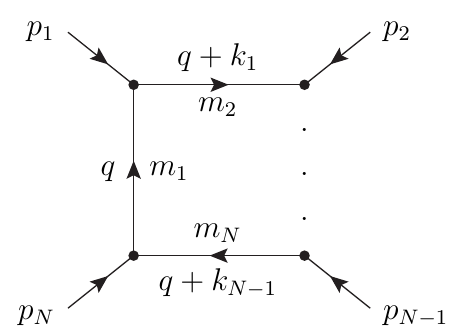
\includegraphics[scale=0.55]{n-points-diagram2}
\caption{General One-loop diagram. \textit{LoopTools}'s convention~\cite{Hahn:1998yk}.}
\end{figure}

The n-point tensor integral in the \textit{LoopTools}'s convention~\cite{Hahn:1998yk} is:
\begin{align}
\label{eq:n-point-integral}
T^N_{\mu_{1}\cdots\mu_{P}}(k_i)=&\dfrac{\mu^{4-D}}{i\pi^{D/2}r_{\Gamma}}\int d^Dq \dfrac{q_{\mu_1}\cdots q_{\mu_P}}{[q^2-m_1^2][(q+k_1)^2-m_2^2]\cdots[(q+k_{N-1})^2-m_{N}^2]}\,,
\end{align} 
with
\begin{align}
r_{\Gamma}=\dfrac{\Gamma^2(1-\epsilon)\Gamma(1+\epsilon)}{\Gamma(1-2\epsilon)}\hspace{1.0 cm} D=4-2\epsilon \,,
\end{align} 
\label{eq:ptok}
where the momenta $k_i$ that appear in the denominators are related to the external momenta $p_i$ as
\begin{align}
p_1=& k_1 \hspace{1 cm} p_2=k_2-k_1 \hspace{1 cm} \cdots \hspace{1 cm} p_N=k_N-k_{N-1}\nonumber \\
k_1=& p_1 \hspace{1 cm} k_2=p_1+p_2 \hspace{1 cm} \cdots \hspace{1 cm} k_N=\sum_{i=1}^N p_i\,.
\end{align}
%
In general, the \textit{LoopTools} notation for the n-point integrals is: $A=T^1$, $B=T^2$, $C=T^3$ and $D=T^4$. Therefore, regarding to the Eq.~\eqref{eq:n-point-integral} we have
%
\begin{align}
\label{eq:A-point-integral}
A_0;A_{\mu}\left(m^2 \right)=&\dfrac{\mu^{4-D}}{i\pi^{D/2}r_{\Gamma}}\int d^Dq \dfrac{ 1;q_{\mu} }{[q^2-m^2]} \,,
\end{align} 
%
\begin{align}
\label{eq:B-point-integral}
B_0;B_{\mu};B_{\mu\nu}\left(p_1^2,m_1^2,m_2^2 \right) 
=&\dfrac{\mu^{4-D}}{i\pi^{D/2}r_{\Gamma}}\int d^Dq \dfrac{ 1;q_{\mu};q_{\mu}q_{\nu} }{[q^2-m_1^2][(q+k_1)^2-m_2^2]} \,,
\end{align} 
%
\begin{align}
\label{eq:C-point-integral}
C_0;C_{\mu};C_{\mu\nu};C_{\mu\nu\rho}&\left(p_1^2,p_2^2,(p_1+p_2)^2,m_1^2,m_2^2,m_3^2\right) \nonumber\\
=&\dfrac{\mu^{4-D}}{i\pi^{D/2}r_{\Gamma}}\int d^Dq \dfrac{ 1;q_{\mu};q_{\mu}q_{\nu};q_{\mu}q_{\nu}q_{\rho} }{[q^2-m_1^2][(q+k_1)^2-m_2^2][(q+k_2)^2-m_3^2]} \,,
\end{align} 
%
\begin{align}
\label{eq:D-point-integral}
D_0;D_{\mu};D_{\mu\nu};D_{\mu\nu\rho};D_{\mu\nu\rho\sigma}&\left(p_1^2,p_2^2,p_3^2,p_4^2,(p_1+p_2)^2,(p_2+p_3)^2,m_1^2,m_2^2,m_3^2,m_4^2\right) \nonumber\\
=&\dfrac{\mu^{4-D}}{i\pi^{D/2}r_{\Gamma}}\int d^Dq \dfrac{ 1;q_{\mu};q_{\mu}q_{\nu};q_{\mu}q_{\nu}q_{\rho};q_{\mu}q_{\nu}q_{\rho}q_{\sigma} }{[q^2-m_1^2][(q+k_1)^2-m_2^2][(q+k_2)^2-m_3^2][(q+k_3)^2-m_4^2]} \,.
\end{align} 
%
They are shown in the Fig.~\ref{fig:n-point-diagrams}.
%
\begin{figure}[h]
\centering
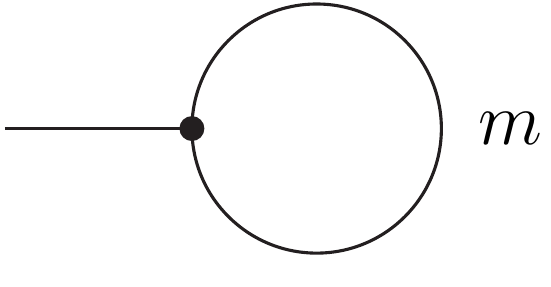
\includegraphics[scale=0.27]{1-points-diagram} \hspace{1 cm}
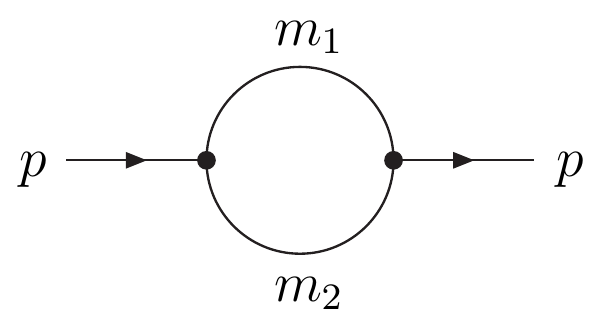
\includegraphics[scale=0.35]{2-points-diagram} 

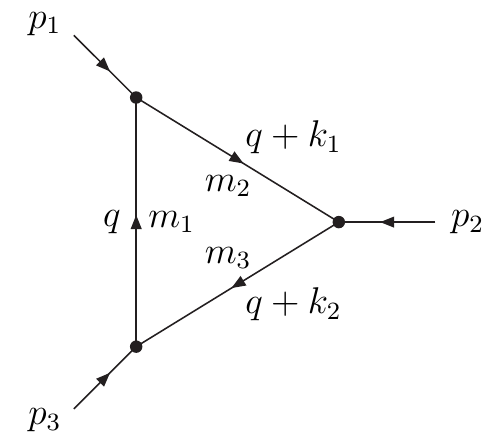
\includegraphics[scale=0.4]{3-points-diagram}\hspace{1 cm}
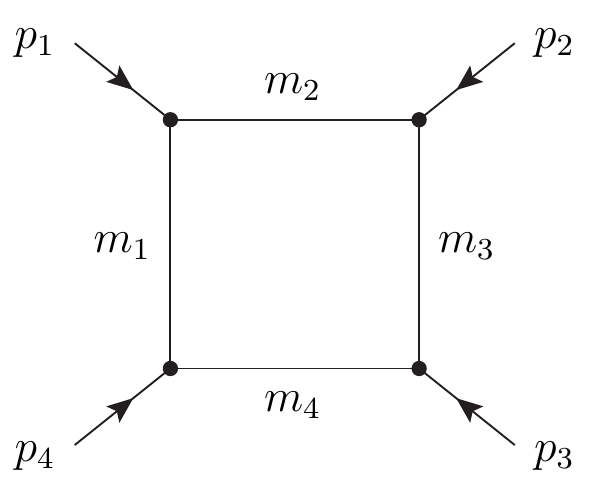
\includegraphics[scale=0.3]{4-points-diagram}
\caption{$A$, $B$, $C$ and $D$ point functions.}
\label{fig:n-point-diagrams}
\end{figure}



\subsection{Tensor Coefficients}
\label{sec:tensor-coefficients}

$\index{tensor coefficients}%
$\index{Lorentz-covariant tensors}%
The integrals with a tensor structure can be reduced to linear
combinations of Lorentz-covariant tensors constructed from the metric
tensor $g_{\mu\nu}$ and a linearly independent set of the momenta~\cite{Passarino:1978jh}.  The choice of this basis is not unique.

%\index{decomposition}%
\textit{LoopTools} provides not the tensor integrals themselves, but the coefficients of
these Lorentz-covariant tensors.  It works in a basis formed from
$g_{\mu\nu}$ and the momenta $k_i$, which are the sums of the external
momenta $p_i$ (see Eq.~\eqref{eq:ptok})~\cite{Denner:1991kt}.  In this basis
the tensor-coefficient functions are totally symmetric in their indices.
For the integrals up to the four-point function the decomposition reads
explicitly
\begin{align*}
B_\mu &=
	k_{1\mu} B_1\,,
	\displaybreak[0] \\
B_{\mu\nu} &=
	g_{\mu\nu} B_{00} + k_{1\mu} k_{1\nu} B_{11}\,,
	\displaybreak[0] \\[1ex]
C_\mu &=
	k_{1\mu} C_1 + k_{2\mu} C_2 = \sum_{i=1}^2 k_{i\mu} C_i\,,
	\displaybreak[0] \\
C_{\mu\nu} &=
	g_{\mu\nu} C_{00} + \sum_{i,j=1}^2 k_{i\mu} k_{j\nu} C_{ij}\,,
	\displaybreak[0] \\
C_{\mu\nu\rho} &=
	\sum_{i=1}^2 \bigl(
	g_{\mu\nu} k_{i\rho}
	+ g_{\nu\rho} k_{i\mu}
	+ g_{\mu\rho} k_{i\nu}\bigr) C_{00i}+
	\sum_{i,j,\ell=1}^2 k_{i\mu} k_{j\nu} k_{\ell\rho} C_{ij\ell}\,,
	\displaybreak[0] \\[1ex]
D_\mu &=
	\sum_{i=1}^3 k_{i\mu} D_i\,,
	\displaybreak[0] \\
D_{\mu\nu} &=
	g_{\mu\nu} D_{00} + \sum_{i,j=1}^3 k_{i\mu} k_{j\nu} D_{ij}\,,
	\displaybreak[0] \\
D_{\mu\nu\rho} &=
	\sum_{i=1}^3\bigl(
	g_{\mu\nu} k_{i\rho}
	+ g_{\nu\rho} k_{i\mu}
	+ g_{\mu\rho} k_{i\nu}\bigr) D_{00i}
	+ \sum_{i,j,\ell=1}^3 k_{i\mu} k_{j\nu} k_{\ell\rho} D_{ij\ell}\,,
	\displaybreak[0] \\
D_{\mu\nu\rho\sigma} &=
	(g_{\mu\nu} g_{\rho\sigma}
	+ g_{\mu\rho} g_{\nu\sigma}
	+ g_{\mu\sigma} g_{\nu\rho}) D_{0000} \\
	& \hphantom{=} + \sum_{i,j=1}^3 \bigl(
	g_{\mu\nu} k_{i\rho} k_{j\sigma}
	+ g_{\nu\rho} k_{i\mu} k_{j\sigma}
	+ g_{\mu\rho} k_{i\nu} k_{j\sigma} \\[-1.5ex]
	& \hphantom{=+\sum_{i,j=1}^3\bigl(\,}
	+ g_{\mu\sigma} k_{i\nu} k_{j\rho}
	+ g_{\nu\sigma} k_{i\mu} k_{j\rho}
	+ g_{\rho\sigma} k_{i\mu} k_{j\nu}\bigr) D_{00ij} \\[-1ex]
	& \hphantom{=} + \sum_{i,j,\ell,m=1}^3
	k_{i\mu} k_{j\nu} k_{\ell\rho} k_{m\sigma} D_{ij\ell m}\,.
\end{align*}
Of all scalar and tensor-coefficient functions implemented in \textit{LoopTools}, only 
$A_0$, $B_0$, $B_1$, $B_{00}$, $B_{11}$, $B_{001}$, $B_{111}$, $B'_{00}$,
the C coefficients with at least two indices zero, and the D coefficients
with at least four indices zero are actually UV divergent~\cite{Hahn:1998yk}.


\subsection{Conventions for the Momenta}

%\index{momenta!conventions for}%
A large source of mistakes is the way of specifying the momenta in the
one-loop integrals.  The prime error in this respect is the confusion of
the external momenta $p_i$ with the momenta $k_i$ appearing in the
denominators, which are the sums of the $p_i$ (see Eq.~\eqref{eq:ptok}).

The arguments are given in the conventions of \textit{LoopTools}~\cite{Hahn:1998yk}.
It is however important to realize that \textit{LoopTools} functions like $C_1$ and
$C_{112}$ are the coefficients respectively of $k_{1\mu}$ and $k_{1\mu}
k_{1\nu} k_{2\rho}$, not of $p_{1\mu}$ and $p_{1\mu} p_{1\nu} p_{2\rho}$.






%%%%%%%%%%%%%%%%%%%%%%%%%%%%%%%%%%%%%%%%%%%%%%%%%%%%%%%%%%%%%%%%%%%%%%%%%%%%%%%%%%%%%%%%%%%%%%%%%%%%%
\subsection{$C$ and $D$ reduction to scalar integrals}
\label{sec:CD-reduction}

The original Passarino Veltman squema~\cite{Passarino:1978jh} is based in the assumption of independent external momenta $p_i$. When the momenta are linearly dependent the Gram Determinant of the momenta goes to zero and the Passarino Veltamann schema breaks down. In that case, we can deal with this problem reducing the n-point integrals to a linear combination of $(n-1)$-point integrals as we will describe.
  
In general, the n-point scalar integral is:
\begin{align}
\label{eq:n-point-scalar}
T^N_0(k_i)=&\dfrac{\mu^{4-D}}{i\pi^{D/2}r_{\Gamma}}\int d^Dq \dfrac{1}{[q^2-m_1^2][(q+k_1)^2-m_2^2]\cdots[(q+k_{N-1})^2-m_{N}^2]}\nonumber\\
=&\dfrac{\mu^{4-D}}{i\pi^{D/2}r_{\Gamma}}\int d^Dq \dfrac{1}{N_1N_2\cdots N_N}\,,
\end{align} 
with
\begin{align}
N_i=& (q+k_{i-1})^2-m_i^2 \,, \hspace{1 cm} i=1,\cdots N \hspace{1 cm} k_0=0\,.
\end{align}
In the case of degeneration in the momenta, $T^N_0(k_i)$ can be expanded by $T^{N-1}_0(k_i)$ in the next form:
%
\begin{align}
\label{eq:int-reduction}
T_0^N=\sum_{i=1}^{N}\alpha_i\left(\dfrac{\mu^{4-D}}{i\pi^{D/2}r_{\Gamma}}\int d^Dq \dfrac{1}{N_1N_2\cdots N_{i-1}N_{i+1}\cdots N_N}\right)
=\sum_{i=1}^{N}\alpha_i\,T_0^{N-1}(i)\,.
\end{align}
In order to know the necessary condition to find the $\alpha_i$ coefficients we can use the Eq.~\eqref{eq:n-point-scalar} and \eqref{eq:int-reduction}. In means that we  have to fulfill
\begin{align}
\dfrac{1}{N_1N_2\cdots N_N}= \dfrac{\alpha_1}{N_2N_3\cdots N_N}+\dfrac{\alpha_2}{N_1N_3\cdots N_N}+\cdots +\dfrac{\alpha_N}{N_1N_2N_3\cdots N_{N-1}}
=\dfrac{\sum_{i=1}^N\alpha_iN_i}{N_0N_1\cdots N_N}\,,
\end{align}
%
therefore
%
\begin{align}
1=\sum_{i=1}^N\alpha_iN_i=\sum_{i=1}^N\alpha_i(q^2+2q_{\mu}k_{i-1}^{\mu}+k_{i-1}^2-m_{i}^2)
=q^2\sum_{i=1}^N\alpha_i + 2q_{\mu}\sum_{i=1}^N\alpha_ik_{i-1}^{\mu} + \sum_{i=1}^N\alpha_i (k_{i-1}^2-m_i^2)\,.
\end{align}
%
Now, in order to satisfied this condition for all momenta $q_{\mu}$, we have to guaranteed the next three relations:
\begin{align}
\sum_{i=1}^N\alpha_i = 0 \hspace{1 cm}
\sum_{i=1}^N\alpha_ik_{i-1} = 0  \hspace{1 cm}
\sum_{i=1}^N\alpha_i (k_{i-1}^2-m_i^2) =& 1\,.
\end{align}
In particular, the second condition guaranteed that
\begin{align}
\alpha_2k_1+\alpha_3k_2+\alpha_4k_3\cdots \alpha_{N}k_{N-1}=0\,.
\end{align}
%
If the set of momenta $\{k_1, k_2 \cdots k_{N-1}\}$ are $(N-1)$ linear independent, we will have the  trivial solution $\alpha_i=0$ for all $i$. Now, in order to don't have the trivial solution, the $k_i$ momenta must be linearly dependent as our preliminary condition when the Passarino Veltman schema breaks down.

The last schema is general for reduce an $n$-point integral to a $(n-1)$-point integral. We will focus in the particular case of $N=3$ and $N=4$.
%
For $N=3$, the $C$ scalar integral can be reduce to $B$ $(N=2)$ if you satisfied the next three relations
\begin{align}
\sum_{i=1}^N\alpha_i = 0 \hspace{0.5 cm} &\rightarrow \hspace{0.5  cm} \alpha_1+\alpha_2+\alpha_3=0 \\
\sum_{i=1}^N\alpha_ik_{i-1} = 0 \hspace{0.5  cm} &\rightarrow \hspace{0.5  cm} \alpha_2k_1+\alpha_3k_2=\alpha_2p_1+\alpha_3(p_1+p_2)=0 \nonumber \\ 
& \Rightarrow \hspace{0.5  cm} \alpha_2p_1^2+\alpha_3(p_1^2+p_1\cdot p_2)= \alpha_2p_1^2+\alpha_3\dfrac{(p_1^2-p_2^2+p_3^2)}{2}=0 \\
\sum_{i=1}^N\alpha_i (k_{i-1}^2-m_i^2) = 1\hspace{0.5  cm} &\rightarrow \hspace{0.5  cm} 
-\alpha_1m_1^2+ \alpha_2(k_1^2-m_2^2)+ \alpha_3(k_2^2-m_3^2)\nonumber\\
&\hspace{0.6 cm}=-\alpha_1m_1^2+ \alpha_2(p_1^2-m_2^2)+ \alpha_3(p_3^2-m_3^2)=1\,,
\end{align} 
which are summary in the next system of equation:
\begin{align}
\begin{pmatrix}
1 & 1 & 1 \\
0 & p_1^2 & (p_1^2-p_2^2+p_3^2)/2 \\
 -m_1^2 & (p_1^2-m_2^2) & (p_3^2-m_3^2)
\end{pmatrix}
\begin{pmatrix}
\alpha_1 \\ \alpha_2 \\ \alpha_3
\end{pmatrix}=
\begin{pmatrix}
0 \\ 0 \\ 1
\end{pmatrix}\,.
\end{align}
%
Explicitily, according to the Eq.~\eqref{eq:int-reduction}
\begin{align}
\label{eq:t30}
T^3_0=& \left(\dfrac{\mu^{4-D}}{i\pi^{D/2}r_{\Gamma}}\int d^Dq \dfrac{\alpha_1}{N_2N_3}\right)
+\left(\dfrac{\mu^{4-D}}{i\pi^{D/2}r_{\Gamma}}\int d^Dq \dfrac{\alpha_2}{N_1N_3}\right)
+\left(\dfrac{\mu^{4-D}}{i\pi^{D/2}r_{\Gamma}}\int d^Dq \dfrac{\alpha_3}{N_1N_2}\right)\,,
\end{align}
or equivalente:
\begin{align}
C_0(1,2,3)=&\alpha_3B_0(1,2)+\alpha_2B_0(1,3) +\alpha_1B_0(2,3)\nonumber \\
=& \alpha_{12}B_0(1,2)+\alpha_{13}B_0(1,3)+\alpha_{23}B_0(2,3)\,, 
\end{align}
where $C(i,j,k)$ means the $C$ three points functions with denominator $N_iN_jN_k$. The same for $B(i,j)$. Notice that I change the notation for the coefficients $\alpha_i$ in order to get a more compact notation. 

Analogously, for $N=4$, the $D$ scalar integrals can be reduce to $C$ $(N=3)$ scalar integrals and the coefficient can be found solving the next matrix equation
\begin{align}
\begin{pmatrix}
1 & 1 & 1 & 1 \\
0 & p_1^2 & (p_1^2-p_2^2+p_5^2)/2  & (p_1^2+p_4^2-p_6^2)/2\\
0 & (-p_1^2-p_2^2+p_5^2)/2 & (-p_1^2+p_2^2+p_5^2)/2  & (-p_1^2-p_3^3+p_5^2+p_6^2)/2\\
 -m_1^2 & p_1^2-m_2^2 & p_5^2-m_3^2 & p_4^2-m_4^2
\end{pmatrix}
\begin{pmatrix}
\alpha_{234} \\ \alpha_{134} \\ \alpha_{124} \\ \alpha_{123}
\end{pmatrix}=
\begin{pmatrix}
0 \\ 0 \\ 0 \\ 1
\end{pmatrix}\,,
\end{align}
%
with $p_5=p_1+p_2$ and $p_6=p_2+p_3$.\\
The scalar reduction in this case is
\begin{align}
D_0(1,2,3,4)= \alpha_{123}C_0(1,2,3)+\alpha_{124}C_0(1,2,4)+\alpha_{134}C_0(1,3,4)+\alpha_{234}C_0(2,3,4)\,.
\end{align}

For the case of tensor reduction we have to take care of \textit{LoopTools} works in the base of the $k_i$ momenta as we described in the Sec.~\ref{sec:tensor-coefficients}. 

We are interested only in the reduction of the 4-point integrals $D_{\mu}$, $D_{\mu\nu}$,$D_{\mu\nu\rho}$ to 3-point functions, because in general the 3-2-1-point functions have analytically representation that we are able to find. 
For $D_{\mu}$ tensor we have
%
\begin{align}
\label{eq:du}
D_{\mu}\approx &\int d^Dq \dfrac{ q_{\mu} }{[q^2-m_1^2][(q+k_1)^2-m_2^2][(q+k_2)^2-m_3^2][(q+k_3)^2-m_4^2]}
=\int d^Dq \dfrac{ q_{\mu} }{[1][2][3][4]} \nonumber \\
=&\alpha_{123}\int d^Dq \dfrac{ q_{\mu} }{[1][2][3]} 
+\alpha_{124}\int d^Dq \dfrac{ q_{\mu} }{[1][2][4]} 
+\alpha_{134}\int d^Dq \dfrac{ q_{\mu} }{[1][3][4]} 
+\alpha_{234}\int d^Dq \dfrac{ q_{\mu} }{[2][3][4]}\,. 
\end{align} 
%
We omit the factor $\dfrac{\mu^{4-D}}{i\pi^{D/2}r_{\Gamma}}$ in the last equation in order to have a more compact notation. To continue, we have to take some care with the last integral. It does not have the canonical definition of the three point functions because the first propagator has an external momenta $k_1=p_1$. In order to have the canonical definition we can do a simple change of variable $q+k_1\rightarrow q^{'}$ 
\begin{align}
\label{eq:c234}
\int d^Dq \dfrac{ q_{\mu} }{[2][3][4]}=&\int d^Dq \dfrac{ q_{\mu} }{[(q+k_1)^2-m_2^2][(q+k_2)^2-m_3^2][(q+k_3)^2-m_4^2]}\nonumber \\
=& \int d^Dq \dfrac{ (q_{\mu}-k_{1\mu}) }{[q^2-m_2^2][(q+(k_2-k_1))^2-m_3^2][(q+(k_3-k_1))^2-m_4^2]}\nonumber \\
=& \tilde{C}_{\mu}(2,3,4)-k_{1\mu}\tilde{C}_0(2,3,4)\,,
\end{align}
where the tilde means that we have to take care with the last shift in the propagator's momenta.

Replacing the Eq.~\eqref{eq:c234} in the Eq.~\eqref{eq:du} and using the definition of the $C_{\mu}$ tensor, we have
%
\begin{align}
D_{\mu}=& \alpha_{123}C_{\mu}(1,2,3)+\alpha_{124}C_{\mu}(1,2,4)+\alpha_{134}C_{\mu}(1,3,4) +\alpha_{234}\left(\tilde{C}_{\mu}(2,3,4)-k_{1\mu}\tilde{C}_0(2,3,4)\right)\,.
\end{align} 

Finally, using the definition of the tensor coefficients given in the Sec.~\ref{sec:tensor-coefficients} we have that
%
\begin{align}
D_{\mu}=&\alpha_{123}\left(k_{1\mu}C_1(1,2,3)+k_{2\mu}C_2(1,2,3)\right)
+\alpha_{124}\left(k_{1\mu}C_1(1,2,4)+k_{3\mu}C_2(1,2,4)\right)\nonumber \\
+&\alpha_{134}\left(k_{2\mu}C_1(1,3,4)+k_{3\mu}C_2(1,3,4)\right)\nonumber \\
+&\alpha_{234}\left((k_{2\mu}-k_{1\mu})\tilde{C}_1(2,3,4)+(k_{3\mu}-k_{1\mu})\tilde{C}_2(2,3,4)-k_{1\mu}\tilde{C}_0(2,3,4)\right)\,.
\end{align}
%
But for definition $D_{\mu}=k_{1\mu}D_1+k_{2\mu}D_2+k_{3\mu}D_3$, therefore, doing the matching in the momenta $k_i$, we have the relation between the coefficients tensor of $D$ and $C$ functions
\begin{align}
\label{eq:Di-reduction}
D_0=& \alpha_{123}C_0+\alpha_{124}C_0+\alpha_{134}C_0+\alpha_{234}\tilde{C}_0\nonumber \\
D_1=&\alpha_{123}C_1+\alpha_{124}C_1+0*\alpha_{134}C_1-\alpha_{234}\left(\tilde{C}_0+\tilde{C}_1+\tilde{C}_2\right)\nonumber \\
D_2=&\alpha_{123}C_2+0*\alpha_{124}C_1+\alpha_{134}C_1+\alpha_{234}\tilde{C}_1\nonumber \\
D_1=&0*\alpha_{123}C_1+\alpha_{124}C_2+\alpha_{134}C_2+\alpha_{234}\tilde{C}_2\,,
\end{align}
where we included the scalar reduction for $D_0$ found before and a more compact notation $\alpha_{ijk}C_l=\alpha_{ijk}C_l(ijk)$.

Analogically, for $D_{\mu\nu}$ tensor reduction we found

\begin{align}
\label{eq:Dij-reduction}
D_{00}=& \alpha_{123}C_{00}+\alpha_{124}C_{00}+\alpha_{134}C_{00}+\alpha_{234}\tilde{C}_{00}\nonumber \\
D_{11}=&\alpha_{123}C_{11}+\alpha_{124}C_{11}+0*\alpha_{134}C_1+\alpha_{234}\left(\tilde{C}_0+2\tilde{C}_1+2\tilde{C}_2+\tilde{C}_{11}+2\tilde{C}_{12}+\tilde{C}_{22}\right)\nonumber \\
D_{12}=&\alpha_{123}C_{12}+0*\alpha_{124}C_{22}+0*\alpha_{134}C_{22}-\alpha_{234}\left(\tilde{C}_{1}+\tilde{C}_{11}+\tilde{C}_{12}\right)\nonumber\\
D_{13}=&0*\alpha_{123}C_{12}+\alpha_{124}C_{12}+0*\alpha_{134}C_{22}-\alpha_{234}\left(\tilde{C}_{12}+\tilde{C}_{2}+\tilde{C}_{22}\right)\nonumber\\
D_{22}=&\alpha_{123}C_{22}+0*\alpha_{124}C_1+\alpha_{134}C_{11}+\alpha_{234}\tilde{C}_{11}\nonumber \\
D_{23}=&0*\alpha_{123}C_{22}+0*\alpha_{124}C_1+\alpha_{134}C_{12}+\alpha_{234}\tilde{C}_{12}\nonumber \\
D_{33}=&0*\alpha_{123}C_{22}+\alpha_{124}C_{22}+\alpha_{134}C_{22}+\alpha_{234}\tilde{C}_{22}\,,
\end{align}

and for $D_{00i}$ tensor reduction we found

\begin{align}
\label{eq:D00i-reduction}
D_{001} =& \alpha_{123}C_{001}+\alpha_{124}C_{001}+0*\alpha_{134}C_{00}-\alpha_{234}\left(\tilde{C}_{00}+\tilde{C}_{001}+\tilde{C}_{002}\right)\nonumber \\
D_{002} =& \alpha_{123}C_{002}+0*\alpha_{124}C_{001}+\alpha_{134}C_{001}+\alpha_{234}\tilde{C}_{001}\nonumber \\
D_{003} =& 0*\alpha_{123}C_{00}+\alpha_{124}C_{002}+\alpha_{134}C_{002}+\alpha_{234}\tilde{C}_{002}\,.
\end{align}

\noindent
For another and complete reduction of the tensor n-point $T^N_{\mu_1\cdots \mu_{P}}$ integrals but in another base, see~\cite{STUART1988367}. For us, that schema is not useful because \textit{LoopTools} work in the $k_i$ base that is not the base used in the work. 








